% !TEX encoding = UTF-8 Unicode
%!TEX root = ../Main/thesis.tex
% !TEX spellcheck = en-US
%%=========================================
\documentclass[../Main/thesis.tex]{subfiles}
\begin{document}
\chapter{Introduction}
\label{ch:introduction}
%The first chapter of a well-structured thesis is always an introduction, setting the scene with background, problem description, objectives, limitations, and then looking ahead to summarize what is in the rest of the report. 
%This is the part that readers look at first---\emph{so make sure it hooks them!}

%%=========================================
\section{Background}
\label{sec:background}
%In this section, you should present the problem that you are going to investigate or analyze; why this problem is of interest; what has, so far, been done to solve the problem, and which parts of the problem that remain.
%{\color{red}Below, I have set up some headings (subsection titles) without a number. 
%These are included to help you remember to cover the related issues. 
%The headings should be removed in your final print.}
%%=========================================
%\subsection*{Problem Formulation}
In the associate press, one of the leading news organization, one could read: \say{Norwegian probe: Gearbox failure cause fatal 2016  crash}.
It was a news report of an airbus helicopter crash, on a small island outside of Bergen, the second largest city in Norway, cutting short the life of 13 people. The official cause of the crash: \say{A fatigue fracture in the main rotor gearbox.}. The anticipated question that arrises after such catastrophic event is: was the dram preventable?

Since the industrial revolution, engines and machines have been the driving force for economical growth across industries such as automotive, airline, oil and gas, to name a few. However, machines are prone to failure, and must be monitored and maintained regularly, to avoid catastrophic failure, which can lead inevitably, to human life and significant financial lost. 
\justify
To mitigate equipment and machines proclivity toward failure and the associated cost, a process called predictive maintenance has been developed within the industrial community. Predictive maintenance  for machines and industrial equipments can be defined as a maintenance philosophy or more generally a framework, with a set of standards and methods, used to predict and prevent machine failure. This maintenance philosophy, when correctly implemented, increases machine life time, reduces downtime and maintenance cost. The aim here, is to detect as early as possible onset of failure and take appropriate actions.
\justify
In rotating machines such as gearbox, more than $40 \% $ of failure can be attributed to bearing faults \cite{albrecht1986}, as shown in figure \ref{fig:pie}. By facilitating rotation movements, bearings can be subjected to large load and mechanical forces, which can lead to slowly propagating defect. The most commonly applied method in predictive maintenance for bearing faults detection, is a Fast Fourier Transform (FFT) based method. The latter consists of decomposing a vibration signal emanating from a bearing, to its corresponding frequency spectrum, through trigonometric basis functions. If the bearing exhibits signs of failure, the fundamental frequencies, which are the failure frequencies, will be consistently visible in the frequency spectrum. It is worth noting that, a bearing failure frequency is derived from its physical characteristics, and depends on the rotating speed of the machine housing the bearings.

\begin{figure}[H] %  figure placement: here, top, bottom, or page
   \centering
   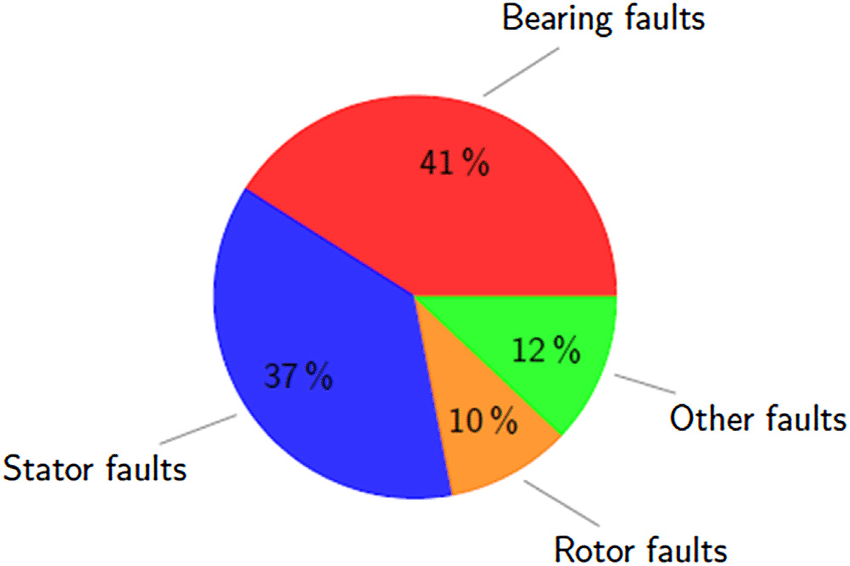
\includegraphics[width=4in]{../fig/pie.png} 
   \caption{Failure distribution in a rotating machine. }
   \label{fig:pie}
\end{figure}
\justify
The Fourier transform based method for bearing fault detection, although efficient, presents some limitations.
 For constant machine rotating speed, it is straight forward to estimate the fundamental frequencies. However, when the rotating speed varies continuously, it can be challenging to estimate the failure frequencies accurately, and this can lead to incorrect fault diagnosis. In addition, the trigonometric basis functions are not compactly supported, hence, an inability to capture local events in a signal.
\justify
To circumvent the latter, many efforts have been directed toward alternative methods for bearing fault detection. In this thesis, we focused on methods derived from Hilbert Huang transform, wavelet transform and machine learning. The attractiveness of these methods lies on the key fact of not requiring the bearing physical characteristics, and the rotating speed of the machine, in order to detect failure. The Hilbert Huang and the wavelet transform, by construct, can reveal local phenomenon in a signal.
\justify
Hilbert Huang transform was developed recently by  Huang, \cite{huang98} to deal efficiently with non linear and non stationary processes. It decomposes data adaptively 
into its sub-components by using the so called empirical mode decomposition (EMD). Unlike Fourier transform where trigonometric functions are used to decomposed signals, adaptive decomposition means that 
the basis functions are completely determined by the data itself, \cite{huang08}. This allows in theory, to access intrinsic and salient properties of data.
\justify
Wavelet transform is a signal analysis tool such as Fourier transform. In contrast to the latter, wavelets can be used to detect short duration hight frequency burst, \cite{albert09}.
Wavelets are family of functions generated by two functions: the so called mother wavelet and a scaling function. The scaling property allows a wavelet to zoom in, on short and high frequency pulses \cite{albert09},
such as tiny onset of cracks in bearings.
\justify
Machine learning methods commonly used are supervised and unsupervised learning methods. In supervised learning, an algorithm learns the pattern of instances of failure, in order to detect them in subsequent samples. It is however common that failure instances are not available or are too scarce to learn from. In that event, unsupervised learning algorithms are the alternative to supervised learning. The former categorizes data into different groups where data points in the same cluster share some sort of similarity.
\justify
 The application of the aforementioned methods for bearing failure detection, have been studied by various researchers. 
To set apart this work from what has been previously achieved, we present a literature survey in section \ref{sec:relatedwork}, followed by our contribution in section \ref{sec:contributions}. Since Fourier transform based method is the standard for bearing fault detection across various industries, chapter \ref{sec:chapter2} shows how Fourier analysis is applied to bearing fault detection by using a concrete case study. This will serve as a reference with regards to Hilbert Huang transform, wavelet transform and machine learning methods.
\justify
Chapter \ref{sec:hht} and \ref{sec:waveletandsvm} cover the contribution of this work. In Chapter \ref{sec:hht}, we show how Hilbert Huang transform coupled with a robust seasonal trend decomposition method, can detect high frequency and short duration pulses, generated by bearing faults. In chapter \ref{sec:waveletandsvm} we present a methodology to quantify bearings health and classify multiples bearings with wavelet transform and machine learning. Chapter \ref{ch:conclusions} presents the conclusion of the thesis through a summary, and pinpoint some of its limitations. To improve upon what has be achieved in this thesis have, a road map with suggestions is outlined.

%The detailed treatment of these methods and the 
%%=========================================
\section{Related work}
\label{sec:relatedwork}
The widely applied method for bearing fault detection in most industries, is based on Fourier transform (\cite{gupta2016}, \cite{khadersab2018}, \cite{randal2010}). In the latter, a snapshot vibration signal obtained from a bearing, is decomposed into its elementary parts, which constitutes the frequency spectrum. Furthermore, any failure incur by a bearing will induce a specific frequency, which, inevitably can be found in the frequency spectrum.
\justify
Although powerful, the Fourier transform method is not without its limitations, which have been presented in section \ref{sec:background}. To extend bearing fault detection to cases where the Fourier transform based method is limited,
numerous contributions have been made towards alternative methods such as Hilbert Huang transform, wavelet transform and machine learning (\cite{zhang2019}, \cite{xiaoan2018}, \cite{rai2016}, \cite{konar2011}, \cite{rai2006} ).
\justify
The Hilbert Huang transform as most signal analysis tool, is predicated on the assumption that a signal has multiple components and can be decomposed into single oscillatory modes called intrinsic mode functions (IMFs). 
(\cite{fan2016}) decomposed the vibration signal obtained from a motor into intrinsic mode functions, and evaluated the Hilbert Huang energy spectrum of each IMF, to detect sign of fatigue, oxidation and mechanical structure deformation. The energy spectrum also called power spectrum or energy density, is the energy contribution of each frequency, derived from the intrinsic mode functions.
To compute the energy density, the Hilbert transform of the absolute value of the square of an IMF is first computed. Secondly, the integral of the latter is evaluated over the domain of variability of the signal. The Hilbert transform of a signal is the convolution of the signal with the function $\frac{1}{\pi t}$, where $t$ is a dummy variable.
\justify
One of the issue of the Hilbert Huang transform, is selecting the appropriate intrinsic mode functions. The IMFs obtained from a target signal, are hierarchy of mono component signals, ranging from high to low frequency. For a given process such as the vibration of a bearing in a motor, there exists multiple sub processes corresponding to the vibration of sub components of the motor and the bearing. Therefore mapping the correct IMFs to the corresponding sub processes is a daunting task. To resolve this issue, (\cite{osman2013a}, \cite{osman2013b} ) used a linear combination of two similarities measure (Linear and non-linear similarity) to select the target IMF and applied the energy spectrum of the IMFs to identify bearing failure frequencies. The similarities measures, quantifies the \say{sameness} of two distributions.
In the same fashion (\cite{osman2014}) applied a weighted D'Agostino Pearson (DP) normality test to select the more relevant IMFs (IMF representing defect component). The DP test uses both the skewness and the kurtosis to assess normality.
The skewness is a statistical estimator that measures the symmetry of a probability distribution, while the kurtosis also a statistical estimator, measures the \say{tailedness} of a distribution. The Kurtosis and skewness of a normal distribution are 3 and 0 respectively.
Most of the Hilbert Huang transform methods applied to bearing fault detection uses the energy spectrum of the IMFs to identify the bearing failure frequencies (more citation here).
\justify
One of the machine learning method for bearing fault detection is the Support Vector Machine (SVM). It is a linear classification algorithm that separates similar data points into different groups (\cite{vapnik1995}). The data points are  often displayed in a two dimensional reference frame, where the classification takes place. The reference frame is often called the feature space, because its axis are ranges of some statistical estimators. (\cite{konar2011}) applied wavelet transform to decomposed a vibration signal from a bearing and estimated the root mean square, the crest factor and the kurtosis. The former to the latter are the features used to classify bearing fault with a support vector machine. Using a transform to extract signals for classification is called feature extraction. (\cite{singh2018}) used Stockwell transform for feature extraction in a support vector machine classification. Other statistical estimator used as features in a support vector machine classification are the range, the mean value the standard deviation. Except the former, all others statistical estimator are not robust in the sens that they are sensitive to outliers. (\cite{kankar2010}) directly estimated the range, the mean, the standard deviation, the skewness, the kurtosis and the crest factor of bearing vibration signals, and applied a support vector machine for bearing fault classification.
\justify
The main approaches for the application of Hilbert Huang transport for bearing fault detection is based on decomposing a bearing vibration signal into intrinsic mode function (IMFs). Furthermore, the IMFs energy spectrum are used to detect the bearing failure frequencies. These methods are frequency based and ignore the time signal of the IMFs.
\justify
The application of support vector machine in bearing fault detection requires at least two features derived from the bearing vibration signal. The features are most often statistical estimators. In most cases they are (statistical) moment that measure the shape of a (distribution) signal. These estimators are often not robust, which make them sensitive to outliers. The measurement of vibration signals are often contaminated with measurement errors that generate outliers. In addition, for a nonlinear and non-stationary process such as a motor changing continuously load, outliers are not sign of anomalies. To address these issues two methods are presented in this thesis. 




%%=========================================

\section{Contributions }
\label{sec:contributions}
The contribution of this work can be summed up in three parts. Firstly, the Hilbert Huang transform coupled with the robust seasonal trend estimation based of Loess [ref], can extract high frequency spikes emitted when bearing balls pass defect area or cracks.
\justify
secondly, the health of a bearing is estimated by a robust statistical dispersion measure: the interquartile range (IQR). The latter is the health index. Furthermore,  the health index is used to estimate a bearing health trajectory. The health trajectory is the different stages a bearing can go through until failure occurs. We show that a bearing can go through three successive phases: The onset of failure, a rapid deterioration and an imminent failure phase. 
\justify
lastly, a health decision boundary is estimated for a system of bearings, based on a wavelet decomposition, the IQR, and a one class support vector machine. A health decision boundary allows for deciding if a bearing is about to fail or not. For each successive vibration signal, a discrete wavelet transform is used to decompose the vibration signal into two new features: The high and low frequency component. The health index of the high and low frequency components are computed. In this fashion, we obtain a set of points in the high and low frequency feature space. By training a one class support vector machine the health decision boundary for multiple bearings is estimated.

%%=========================================

\blankpage
\end{document}
